\documentclass[12pt,a4paper]{article}
\usepackage[utf8]{inputenc}
\usepackage[margin=1in]{geometry}
\usepackage{graphicx}
\usepackage{tikz}
\usepackage{amsmath}
\usepackage{enumitem}
\usepackage{xcolor}
\usepackage{listings}
\usepackage{hyperref}
\usepackage{fancyhdr}
\usepackage{tcolorbox}
\usepackage{tabularx}
\usepackage{booktabs}

\usetikzlibrary{shapes.geometric, arrows, positioning, fit, backgrounds}

% Define colors
\definecolor{primaryblue}{RGB}{0,102,204}
\definecolor{successgreen}{RGB}{40,167,69}
\definecolor{warningyellow}{RGB}{255,193,7}
\definecolor{dangerred}{RGB}{220,53,69}
\definecolor{lightgray}{RGB}{248,249,250}
\definecolor{codebg}{RGB}{245,245,245}

% Header and Footer
\pagestyle{fancy}
\fancyhf{}
\lhead{HireSIGHT AI - Complete Pipeline Flow}
\rhead{Page \thepage}
\renewcommand{\headrulewidth}{0.4pt}

% Title Page
\title{\textbf{\Huge HireSIGHT AI} \\[0.5cm] 
\Large Complete Pipeline Flow \\[0.3cm]
\large From Job Application to Hiring Decision}
\author{Enhanced Evaluation System Documentation}
\date{\today}

% Code Listing Style
\lstset{
    backgroundcolor=\color{codebg},
    basicstyle=\ttfamily\small,
    breaklines=true,
    frame=single,
    numbers=left,
    numberstyle=\tiny\color{gray},
    showstringspaces=false
}

\begin{document}

\maketitle
\newpage

\tableofcontents
\newpage

% ============================================================
\section{Executive Summary}
% ============================================================

\begin{tcolorbox}[colback=primaryblue!5,colframe=primaryblue,title=\textbf{System Overview}]
\textbf{HireSIGHT AI} is an intelligent interview evaluation system that assesses candidates across \textbf{4 dimensions}:

\begin{itemize}[leftmargin=*]
    \item \textbf{Technical} (35\%) - Knowledge \& problem-solving
    \item \textbf{Communication} (25\%) - Vocal confidence \& clarity
    \item \textbf{Behavioral} (20\%) - Eye contact, posture, engagement
    \item \textbf{Coding} (20\%) - Algorithm correctness \& code quality
\end{itemize}

\textbf{Output:} Automated hiring recommendation (Strong Hire / Hire / Maybe / No Hire)
\end{tcolorbox}

\subsection{Key Technologies}
\begin{itemize}
    \item \textbf{MediaPipe:} Facial landmark detection \& behavioral analysis
    \item \textbf{OpenSMILE:} Acoustic feature extraction \& voice analysis
    \item \textbf{Vosk:} Offline speech-to-text recognition
    \item \textbf{Librosa:} Audio processing \& vocal analysis
    \item \textbf{BERT-NER:} Resume parsing \& entity extraction
    \item \textbf{Groq/Grok LLM:} Answer evaluation \& question generation
    \item \textbf{FastAPI:} Backend REST API
    \item \textbf{MongoDB:} NoSQL database
    \item \textbf{Next.js:} Frontend React framework
\end{itemize}

% ============================================================
\section{Complete Pipeline Overview}
% ============================================================

\begin{figure}[h!]
\centering
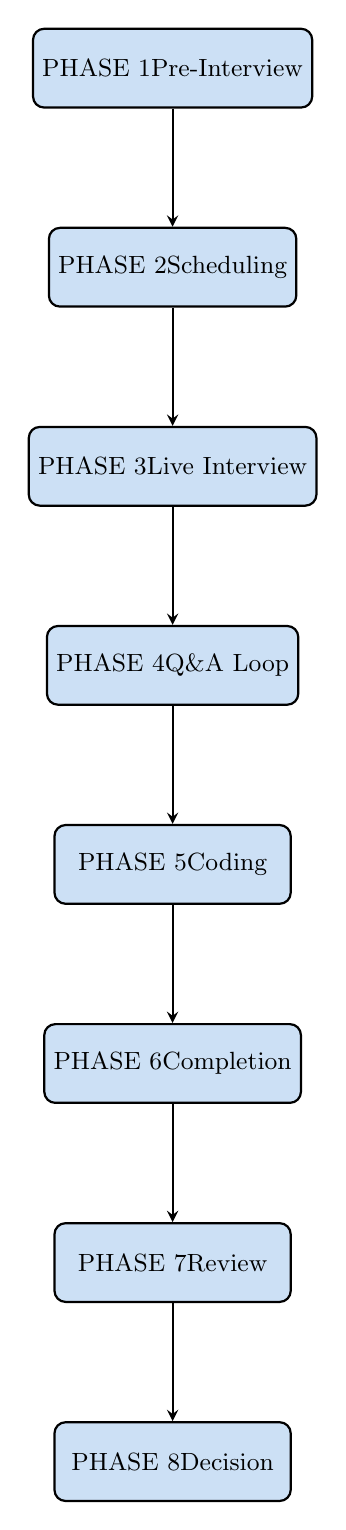
\begin{tikzpicture}[
    node distance=1.5cm,
    every node/.style={font=\small},
    phase/.style={rectangle, rounded corners, minimum width=3cm, minimum height=1cm, 
                  text centered, draw=black, fill=primaryblue!20, thick},
    step/.style={rectangle, minimum width=2.8cm, minimum height=0.8cm,
                 text centered, draw=black, fill=white, thick},
    arrow/.style={->, >=stealth, thick}
]

% Phases
\node (phase1) [phase] {PHASE 1\\Pre-Interview};
\node (phase2) [phase, below=of phase1] {PHASE 2\\Scheduling};
\node (phase3) [phase, below=of phase2] {PHASE 3\\Live Interview};
\node (phase4) [phase, below=of phase3] {PHASE 4\\Q\&A Loop};
\node (phase5) [phase, below=of phase4] {PHASE 5\\Coding};
\node (phase6) [phase, below=of phase5] {PHASE 6\\Completion};
\node (phase7) [phase, below=of phase6] {PHASE 7\\Review};
\node (phase8) [phase, below=of phase7] {PHASE 8\\Decision};

% Arrows
\draw [arrow] (phase1) -- (phase2);
\draw [arrow] (phase2) -- (phase3);
\draw [arrow] (phase3) -- (phase4);
\draw [arrow] (phase4) -- (phase5);
\draw [arrow] (phase5) -- (phase6);
\draw [arrow] (phase6) -- (phase7);
\draw [arrow] (phase7) -- (phase8);

\end{tikzpicture}
\caption{8-Phase Pipeline Overview}
\end{figure}

\subsection{Timeline Summary}
\begin{table}[h!]
\centering
\begin{tabular}{|l|l|l|}
\hline
\textbf{Phase} & \textbf{Duration} & \textbf{Key Activities} \\
\hline
Pre-Interview & 5-10 min & Register, resume upload, apply \\
Scheduling & 1-2 days & Admin reviews \& schedules \\
Interview Setup & 2-3 min & Start, face registration \\
Q\&A (17 questions) & 25-35 min & Answer with real-time analysis \\
Coding (3 challenges) & 15-20 min & Write \& test code \\
Report Generation & 2-3 sec & Automated AI report \\
Recruiter Review & 5-10 min & Review \& make decision \\
\hline
\textbf{TOTAL} & \textbf{1-2 days} & Application to decision \\
\hline
\end{tabular}
\caption{Pipeline Timeline}
\end{table}

\newpage

% ============================================================
\section{PHASE 1: Pre-Interview (Resume Submission)}
% ============================================================

\subsection{Step 1: Candidate Registers \& Logs In}

\begin{lstlisting}[language=bash, caption=Registration API]
POST /auth/register
Content-Type: application/json

Request:
{
  "username": "john_doe",
  "email": "john@example.com",
  "password": "SecurePass123!",
  "full_name": "John Doe"
}

Response:
{
  "user_id": "usr_abc123",
  "access_token": "eyJhbGc...",
  "token_type": "bearer"
}
\end{lstlisting}

\textbf{System Actions:}
\begin{itemize}
    \item Hash password with bcrypt
    \item Generate JWT access token
    \item Store user in MongoDB
    \item Return authentication credentials
\end{itemize}

\subsection{Step 2: Candidate Uploads Resume}

\begin{lstlisting}[language=bash, caption=Resume Upload API]
POST /resume/upload
Authorization: Bearer {token}
Content-Type: multipart/form-data

Request:
- file: resume.pdf (or .docx)

Response:
{
  "profile_id": "prof_xyz789",
  "extracted_data": {
    "name": "John Doe",
    "email": "john@example.com",
    "phone": "+1-234-567-8900",
    "skills": ["Python", "JavaScript", "React", "MongoDB"],
    "experience_years": 5,
    "job_titles": ["Software Engineer", "Full Stack Developer"],
    "companies": ["Tech Corp", "StartupXYZ"],
    "education": ["B.S. Computer Science - MIT"],
    "projects": [
      {
        "name": "E-commerce Platform",
        "technologies": ["React", "Node.js", "MongoDB"]
      }
    ],
    "certifications": ["AWS Certified Developer"]
  },
  "resume_score": 85.5
}
\end{lstlisting}

\textbf{BERT-NER Extraction Process:}
\begin{enumerate}
    \item Parse PDF/DOCX using pdfplumber or python-docx
    \item Extract text content
    \item Apply BERT-NER model (yashpwr/resume-ner-bert-v2)
    \item Identify entities:
    \begin{itemize}
        \item PERSON, EMAIL, PHONE
        \item SKILLS, COMPANIES, JOB\_TITLES
        \item EDUCATION, CERTIFICATIONS
        \item PROJECTS, TECHNOLOGIES
    \end{itemize}
    \item Classify skills (Technical vs. Soft)
    \item Calculate experience years
    \item Store in Profile collection
\end{enumerate}

\newpage

\subsection{Step 3: Resume Analysis \& Skill Classification}

\begin{tcolorbox}[colback=successgreen!5,colframe=successgreen,title=\textbf{Skill Classification Algorithm}]
\textbf{Input:} Raw skills list from resume \\
\textbf{Output:} Categorized skills

\textbf{Categories:}
\begin{itemize}
    \item \textbf{Required Skills:} Matched with job posting requirements
    \item \textbf{Experienced Skills:} Mentioned in work experience section
    \item \textbf{Known Skills:} Mentioned in skills section only
\end{itemize}

\textbf{Scoring:}
\begin{equation}
\text{Resume Score} = \frac{\text{Skills Matched}}{\text{Total Required Skills}} \times 70 + \frac{\text{Experience Years}}{10} \times 30
\end{equation}
\end{tcolorbox}

\subsection{Step 4: Candidate Browses Jobs}

\begin{lstlisting}[language=bash, caption=Job Listings API]
GET /jobs/list?role=Software Engineer&location=Remote

Response:
{
  "jobs": [
    {
      "job_post_id": "job_def456",
      "title": "Senior Software Engineer",
      "company": "TechCorp Inc.",
      "location": "Remote",
      "description": "We are looking for...",
      "required_skills": ["Python", "React", "MongoDB", "AWS"],
      "experience_years": "3-5",
      "salary_range": "$100k - $150k",
      "skill_match": 85.5
    }
  ]
}
\end{lstlisting}

\subsection{Step 5: Candidate Applies to Job}

\begin{lstlisting}[language=bash, caption=Job Application API]
POST /jobs/job_def456/apply
Authorization: Bearer {token}

System Process:
1. Match candidate skills with job requirements
2. Calculate skill match percentage
3. Determine interview eligibility
4. Store application in database
5. Notify admin

Response:
{
  "application_id": "app_ghi789",
  "status": "pending_review",
  "skill_match": 85.5,
  "interview_eligible": true,
  "message": "Application submitted successfully"
}
\end{lstlisting}

\newpage

% ============================================================
\section{PHASE 2: Interview Scheduling}
% ============================================================

\subsection{Step 6: Admin Reviews Application}

\begin{lstlisting}[language=bash, caption=Admin Application Review]
GET /admin/applications
Authorization: Bearer {admin_token}

Response:
{
  "applications": [
    {
      "application_id": "app_ghi789",
      "candidate_name": "John Doe",
      "job_title": "Senior Software Engineer",
      "resume_score": 85.5,
      "skill_match": 85.5,
      "experience_years": 5,
      "status": "pending_review",
      "applied_date": "2025-01-15T10:30:00Z"
    }
  ]
}
\end{lstlisting}

\textbf{Admin Dashboard Features:}
\begin{itemize}
    \item View all pending applications
    \item Filter by skill match, experience, score
    \item Review candidate profile \& resume
    \item Approve/Reject for interview
    \item Schedule interview slots
\end{itemize}

\subsection{Step 7: Interview Scheduled}

\begin{lstlisting}[language=bash, caption=Schedule Interview API]
PUT /admin/applications/app_ghi789/schedule-interview
Authorization: Bearer {admin_token}

Request:
{
  "interview_date": "2025-01-20T14:00:00Z",
  "interview_link": "https://hiresight.ai/interview/xyz",
  "notes": "Technical + Behavioral round"
}

Response:
{
  "status": "interview_scheduled",
  "message": "Candidate notified via email"
}
\end{lstlisting}

\textbf{System Actions:}
\begin{itemize}
    \item Update application status
    \item Send email notification to candidate
    \item Generate interview session link
    \item Add to interview calendar
\end{itemize}

\newpage

% ============================================================
\section{PHASE 3: Live Interview Start}
% ============================================================

\subsection{Step 8: Candidate Starts Interview}

\begin{lstlisting}[language=bash, caption=Start Interview API]
POST /interview/live/start
Authorization: Bearer {token}

Request:
{
  "job_post_id": "job_def456",
  "candidate_name": "John Doe",
  "num_questions": 20
}

System Generates 20 Questions:
- 2 Introduction/Icebreaker
- 7 Technical (based on job role)
- 4 Behavioral (STAR method)
- 4 CV-based (about resume)
- 3 Coding challenges

Response:
{
  "session_id": "int_xyz789",
  "questions": [
    {
      "question_id": "q_1",
      "question_index": 0,
      "question_text": "Tell me about yourself",
      "question_type": "introduction",
      "stage": "introduction"
    },
    {
      "question_id": "q_2",
      "question_index": 1,
      "question_text": "Explain REST API principles",
      "question_type": "technical",
      "stage": "technical",
      "difficulty": "medium"
    },
    // ... 18 more questions
  ]
}
\end{lstlisting}

\textbf{Question Generation Algorithm (LLM):}
\begin{enumerate}
    \item Analyze job role \& description
    \item Review candidate skills \& experience
    \item Review candidate projects \& certifications
    \item Generate personalized questions
    \item Balance difficulty levels (easy/medium/hard)
    \item Ensure coverage of all required skills
    \item Add CV-specific questions about resume
\end{enumerate}

\subsection{Step 9: Face Registration}

\begin{lstlisting}[language=bash, caption=Face Registration API]
POST /interview/live/int_xyz789/register-face
Authorization: Bearer {token}

Request:
{
  "image_base64": "iVBORw0KGgoAAAANSUhEUg..."
}

System Process (DeepFace):
1. Detect face in image
2. Extract facial embeddings (512-dim vector)
3. Store embeddings in database
4. Used for verification during interview

Response:
{
  "registered": true,
  "message": "Face registered successfully"
}
\end{lstlisting}

\newpage

% ============================================================
\section{PHASE 4: Answering Questions (Loop)}
% ============================================================

\subsection{Question-Answer Flow}

\begin{figure}[h!]
\centering
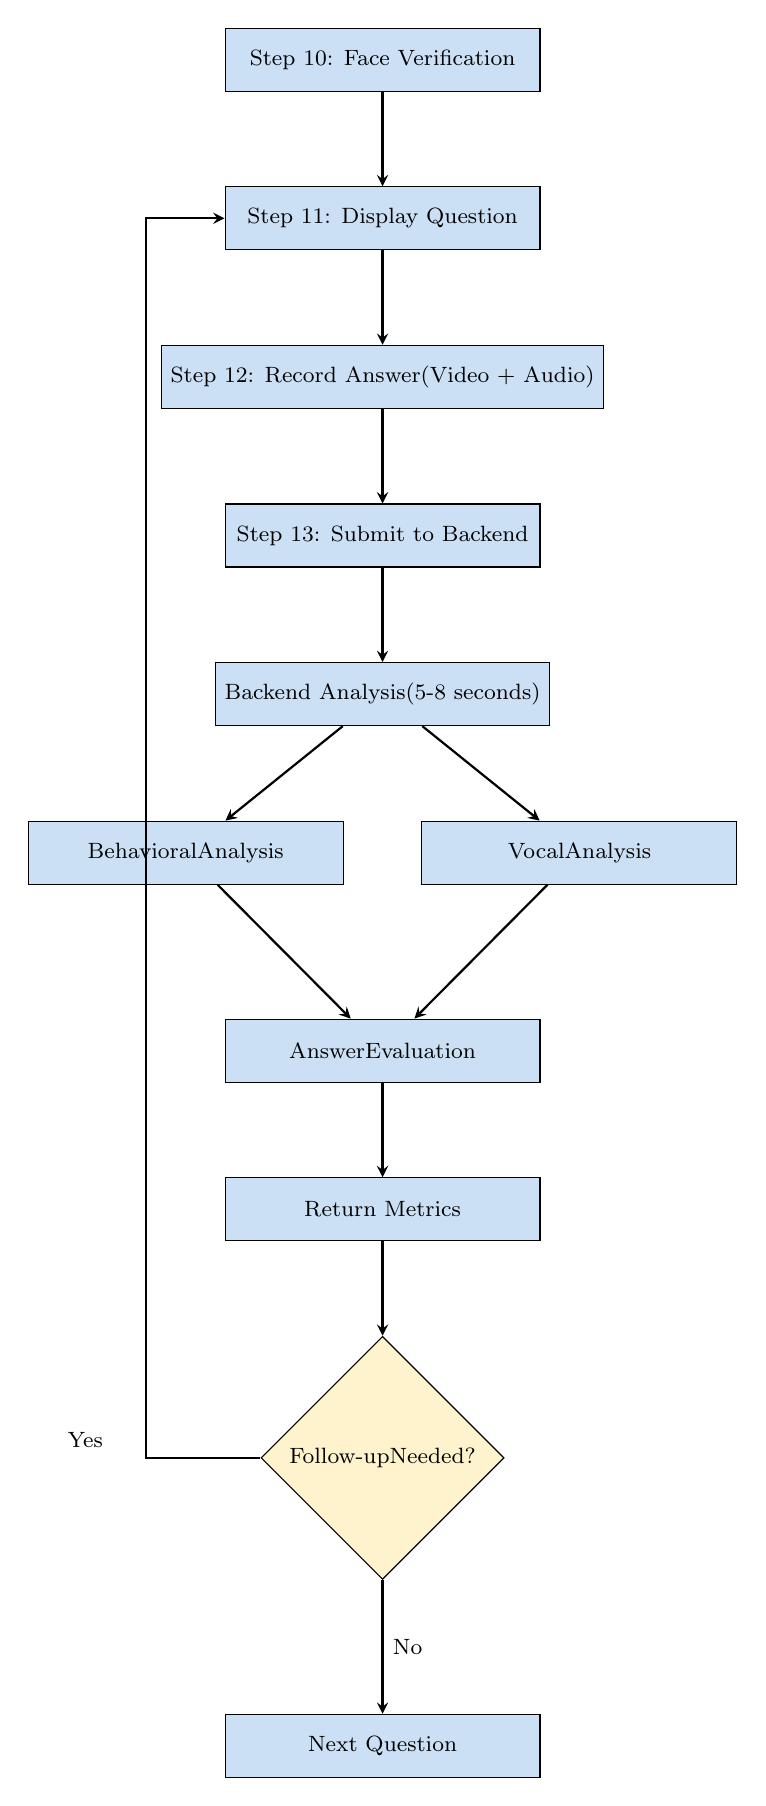
\begin{tikzpicture}[
    node distance=1.2cm,
    every node/.style={font=\footnotesize},
    process/.style={rectangle, minimum width=4cm, minimum height=0.8cm,
                    text centered, draw=black, fill=primaryblue!20},
    decision/.style={diamond, minimum width=2cm, minimum height=1cm,
                     text centered, draw=black, fill=warningyellow!20},
    arrow/.style={->, >=stealth, thick}
]

\node (verify) [process] {Step 10: Face Verification};
\node (display) [process, below=of verify] {Step 11: Display Question};
\node (record) [process, below=of display] {Step 12: Record Answer\\(Video + Audio)};
\node (submit) [process, below=of record] {Step 13: Submit to Backend};
\node (analyze) [process, below=of submit] {Backend Analysis\\(5-8 seconds)};
\node (behavioral) [process, below=of analyze, xshift=-2.5cm] {Behavioral\\Analysis};
\node (vocal) [process, below=of analyze, xshift=2.5cm] {Vocal\\Analysis};
\node (evaluation) [process, below=of behavioral, yshift=-0.5cm, xshift=2.5cm] {Answer\\Evaluation};
\node (metrics) [process, below=of evaluation] {Return Metrics};
\node (followup) [decision, below=of metrics] {Follow-up\\Needed?};
\node (next) [process, below=of followup, yshift=-0.5cm] {Next Question};

\draw [arrow] (verify) -- (display);
\draw [arrow] (display) -- (record);
\draw [arrow] (record) -- (submit);
\draw [arrow] (submit) -- (analyze);
\draw [arrow] (analyze) -- (behavioral);
\draw [arrow] (analyze) -- (vocal);
\draw [arrow] (behavioral) -- (evaluation);
\draw [arrow] (vocal) -- (evaluation);
\draw [arrow] (evaluation) -- (metrics);
\draw [arrow] (metrics) -- (followup);
\draw [arrow] (followup) -- node[right] {No} (next);
\draw [arrow] (followup) -- node[above, xshift=-1.5cm] {Yes} ++(-3,0) |- (display);

\end{tikzpicture}
\caption{Question-Answer Loop Flow}
\end{figure}

\subsection{Step 10: Face Verification}

\begin{lstlisting}[language=bash, caption=Face Verification During Interview]
POST /interview/live/int_xyz789/verify-face

Request:
{
  "image_base64": "iVBORw0KGgoAAAANSUhEUg..."
}

System Process:
1. Extract embeddings from current frame
2. Compare with registered embeddings
3. Calculate cosine similarity
4. Threshold: > 0.6 = Same person

Response:
{
  "verified": true,
  "confidence": 0.92,
  "message": "Identity verified"
}
\end{lstlisting}

\textbf{Anti-Cheating Measures:}
\begin{itemize}
    \item Face verification every question
    \item Detect multiple faces in frame
    \item Monitor screen switching
    \item Track audio anomalies (coaching detection)
\end{itemize}

\newpage

\subsection{Step 11-12: Question Display \& Recording}

\textbf{Frontend Process:}
\begin{enumerate}
    \item Display question text
    \item Start video recording (capture 3-5 frames)
    \item Start audio recording
    \item Show timer (2-3 minutes per question)
    \item Real-time frame capture every 2-3 seconds
    \item Stop recording when done
\end{enumerate}

\subsection{Step 13: Submit Answer with Multi-Modal Data}

\begin{lstlisting}[language=bash, caption=Submit Answer API (Enhanced)]
POST /interview/live/int_xyz789/answer

Request:
{
  "question_index": 0,
  "audio_base64": "UklGRiQAAABXQVZF...",  // WebM audio
  "transcript_text": "I have 5 years of Python experience...",
  "frame_base64_list": [
    "iVBORw0KGgoAAAANSU...",  // Frame 1 (2 sec)
    "iVBORw0KGgoAAAANSU...",  // Frame 2 (4 sec)
    "iVBORw0KGgoAAAANSU...",  // Frame 3 (6 sec)
    "iVBORw0KGgoAAAANSU...",  // Frame 4 (8 sec)
    "iVBORw0KGgoAAAANSU..."   // Frame 5 (10 sec)
  ],
  "audio_format": "webm",
  "language": "en"
}
\end{lstlisting}

\subsection{Backend Analysis Pipeline (5-8 seconds)}

\begin{tcolorbox}[colback=lightgray,colframe=black,title=\textbf{Multi-Modal Analysis Pipeline}]

\textbf{1. SPEECH-TO-TEXT (STT)} - 1-2 seconds
\begin{itemize}
    \item If transcript\_text provided: Use it
    \item Else: Use Vosk offline STT
    \item Output: Text transcript
\end{itemize}

\textbf{2. BEHAVIORAL ANALYSIS (MediaPipe)} - 0.5-1 second
\begin{itemize}
    \item Process 5 video frames
    \item 468-point facial landmark detection
    \item Head pose estimation (pitch, yaw, roll)
    \item Eye gaze direction \& eye contact
    \item Facial engagement detection
    \item Fidgeting \& movement analysis
    \item Output: 6 scores (0-100 each)
\end{itemize}

\textbf{3. VOCAL ANALYSIS (OpenSMILE + Librosa)} - 1-2 seconds
\begin{itemize}
    \item Extract acoustic features (pitch, energy, ZCR)
    \item Analyze speech rate (words per minute)
    \item Detect pause patterns
    \item Measure tone consistency
    \item Calculate vocal confidence
    \item Output: 7 scores (0-100 each)
\end{itemize}

\textbf{4. ANSWER EVALUATION (LLM - Groq/Grok)} - 2-5 seconds
\begin{itemize}
    \item Analyze answer relevance (0-10)
    \item Assess depth of knowledge (0-10)
    \item Check factual accuracy (0-100)
    \item Evaluate communication (0-10)
    \item Identify key points covered
    \item Detect missed points
    \item Coaching detection (audio anomalies)
    \item Output: AnswerEvaluation object
\end{itemize}

\textbf{5. RED FLAG DETECTION}
\begin{itemize}
    \item Poor eye contact (<40\%)
    \item Low vocal confidence (<50\%)
    \item Weak answer quality
    \item Coaching detected
    \item Excessive fidgeting
    \item Output: List of red flags
\end{itemize}

\textbf{6. FOLLOW-UP GENERATION (if needed)}
\begin{itemize}
    \item Triggered if answer lacks depth
    \item Max 3 per stage, 9 total
    \item Generated by LLM
    \item Inserted at question\_index + 1
    \item Output: Follow-up question (optional)
\end{itemize}

\end{tcolorbox}

\newpage

\subsection{Backend Response with Metrics}

\begin{lstlisting}[language=json, caption=Submit Answer Response (Enhanced)]
Response:
{
  "transcript": "I have 5 years of Python experience working on web applications using Django and Flask. I've built RESTful APIs and worked with MongoDB for data storage.",
  
  "evaluation": {
    "question_index": 0,
    "question_text": "Tell me about your Python experience",
    "question_type": "technical",
    "candidate_transcript": "I have 5 years...",
    "relevance_score": 8.5,
    "depth_score": 7.0,
    "communication_score": 8.0,
    "accuracy_score": 85.0,
    "key_points_covered": [
      "5 years experience",
      "Web applications",
      "Django and Flask",
      "RESTful APIs",
      "MongoDB"
    ],
    "missed_points": [
      "Specific project examples",
      "Performance optimization"
    ],
    "is_correct": true,
    "follow_up_triggered": false,
    "coaching_detected": false,
    "evaluator_notes": "Good answer with relevant experience"
  },
  
  "per_answer_score": 82.5,
  
  "behavioral_metrics": {
    "eye_contact": 78.5,
    "head_stability": 85.0,
    "facial_engagement": 72.0,
    "fidgeting": 88.0,
    "confidence_posture": 82.0,
    "attention_span": 90.0
  },
  
  "vocal_metrics": {
    "vocal_confidence": 80.0,
    "speech_clarity": 85.0,
    "pitch_variance": 75.0,
    "speech_rate": 82.0,
    "pause_pattern": 78.0,
    "tone_consistency": 76.0,
    "communication_effectiveness": 82.5
  },
  
  "follow_up_question": null
}
\end{lstlisting}

\newpage

\subsection{Step 14: Real-Time Metrics Display}

\textbf{Frontend Component: MetricsDashboard.jsx}

\begin{figure}[h!]
\centering
\fbox{\begin{minipage}{0.9\textwidth}
\textbf{Real-Time Metrics Dashboard}

\vspace{0.3cm}

\textbf{Behavioral Metrics:}
\begin{itemize}
    \item Eye Contact: \textcolor{successgreen}{78.5/100} \textcolor{successgreen}{●●●●●●●○○○}
    \item Confidence Posture: \textcolor{successgreen}{82.0/100} \textcolor{successgreen}{●●●●●●●●○○}
    \item Attention Span: \textcolor{successgreen}{90.0/100} \textcolor{successgreen}{●●●●●●●●●○}
    \item Fidgeting: \textcolor{successgreen}{88.0/100} \textcolor{successgreen}{●●●●●●●●●○}
\end{itemize}

\vspace{0.2cm}

\textbf{Vocal Metrics:}
\begin{itemize}
    \item Vocal Confidence: \textcolor{successgreen}{80.0/100} \textcolor{successgreen}{●●●●●●●●○○}
    \item Speech Clarity: \textcolor{successgreen}{85.0/100} \textcolor{successgreen}{●●●●●●●●○○}
    \item Communication: \textcolor{successgreen}{82.5/100} \textcolor{successgreen}{●●●●●●●●○○}
\end{itemize}

\vspace{0.2cm}

\textbf{Per-Answer Score:} \textcolor{successgreen}{\textbf{82.5/100}}

\end{minipage}}
\caption{Real-Time Metrics Dashboard (Frontend)}
\end{figure}

\textbf{Color Coding:}
\begin{itemize}
    \item \textcolor{successgreen}{Green (70-100):} Good performance
    \item \textcolor{warningyellow}{Yellow (50-69):} Needs improvement
    \item \textcolor{dangerred}{Red (0-49):} Poor performance
\end{itemize}

\subsection{Repeat for All Questions}

\textbf{Question Loop:}
\begin{enumerate}
    \item Questions 1-2: Introduction/Icebreaker
    \item Questions 3-9: Technical (with possible follow-ups)
    \item Questions 10-13: Behavioral (STAR method)
    \item Questions 14-17: CV-based (about resume)
    \item Questions 18-20: Coding challenges
\end{enumerate}

Each question goes through the same analysis pipeline, collecting 15+ metrics per question.

\textbf{Total Data Collected:}
\begin{equation}
\text{Total Metrics} = 17 \text{ questions} \times 15 \text{ metrics} = 255+ \text{ data points}
\end{equation}

\newpage

% ============================================================
\section{PHASE 5: Coding Challenges}
% ============================================================

\subsection{Step 15: Coding Question Display}

\textbf{Coding Challenge Structure:}
\begin{lstlisting}[language=json, caption=Coding Challenge Format]
{
  "question_id": "q_18",
  "question_text": "Implement a function to reverse a linked list",
  "question_type": "coding",
  "difficulty": "medium",
  "coding_challenge": {
    "language": "python",
    "starter_code": "def reverseList(head):\n    # Your code here\n    pass",
    "description": "Given the head of a singly linked list...",
    "constraints": [
      "Number of nodes: [0, 5000]",
      "Node values: [-5000, 5000]"
    ],
    "examples": [
      {
        "input": "[1,2,3,4,5]",
        "output": "[5,4,3,2,1]"
      }
    ],
    "test_cases": [
      {
        "stdin": "1 2 3 4 5",
        "expected_stdout": "5 4 3 2 1",
        "description": "Normal case"
      },
      {
        "stdin": "",
        "expected_stdout": "",
        "description": "Empty list"
      },
      {
        "stdin": "1",
        "expected_stdout": "1",
        "description": "Single node"
      }
    ]
  }
}
\end{lstlisting}

\subsection{Step 16: Candidate Writes Code}

\textbf{Frontend Code Editor Features:}
\begin{itemize}
    \item Syntax highlighting
    \item Auto-completion
    \item Language selection (Python, JavaScript, C, C++, Java)
    \item Timer display
    \item Test case preview
    \item Save \& test button
    \item Submit button
\end{itemize}

\textbf{Example Code:}
\begin{lstlisting}[language=python, caption=Candidate Solution]
def reverseList(head):
    """
    Reverse a singly linked list iteratively
    Time: O(n), Space: O(1)
    """
    prev = None
    current = head
    
    while current:
        next_node = current.next
        current.next = prev
        prev = current
        current = next_node
    
    return prev
\end{lstlisting}

\newpage

\subsection{Step 17: Test Code Execution}

\begin{lstlisting}[language=bash, caption=Code Execution API]
POST /interview/coding/run

Request:
{
  "language": "python",
  "source_code": "def reverseList(head):\n    prev = None...",
  "test_cases": [
    {
      "stdin": "1 2 3 4 5",
      "expected_stdout": "5 4 3 2 1",
      "description": "Normal case"
    },
    {
      "stdin": "",
      "expected_stdout": "",
      "description": "Empty list"
    },
    {
      "stdin": "1",
      "expected_stdout": "1",
      "description": "Single node"
    }
  ],
  "timeout_seconds": 5.0
}

Backend Process:
1. Save code to temp file
2. Compile (if C/C++/Java)
3. Run against test cases in sandbox
4. Capture stdout, stderr, exit codes
5. Compare actual vs expected output
6. Clean up temp files

Response:
{
  "compile_success": true,
  "compile_output": "",
  "missing_tools": [],
  "all_passed": true,
  "results": [
    {
      "index": 0,
      "passed": true,
      "stdin": "1 2 3 4 5",
      "expected_stdout": "5 4 3 2 1",
      "actual_stdout": "5 4 3 2 1",
      "stderr": "",
      "exit_code": 0,
      "description": "Normal case",
      "error": null
    },
    {
      "index": 1,
      "passed": true,
      "stdin": "",
      "expected_stdout": "",
      "actual_stdout": "",
      "stderr": "",
      "exit_code": 0,
      "description": "Empty list",
      "error": null
    },
    {
      "index": 2,
      "passed": true,
      "stdin": "1",
      "expected_stdout": "1",
      "actual_stdout": "1",
      "stderr": "",
      "exit_code": 0,
      "description": "Single node",
      "error": null
    }
  ]
}
\end{lstlisting}

\newpage

\subsection{Step 18: Submit Coding Result}

\begin{lstlisting}[language=bash, caption=Submit Coding Result API]
POST /interview/live/int_xyz789/submit-coding-result

Request:
{
  "compile_success": true,
  "all_passed": true,
  "results": [...],
  "passed_count": 3,
  "total_count": 3
}

System Process:
- Store coding result in session
- Calculate coding score
- Track for final report

Response:
{
  "status": "success",
  "message": "Coding result recorded",
  "score": 100.0
}
\end{lstlisting}

\textbf{Coding Score Calculation:}
\begin{equation}
\text{Coding Score} = \frac{\text{Test Cases Passed}}{\text{Total Test Cases}} \times 100
\end{equation}

\textbf{Repeat for 3 Coding Challenges:}
\begin{itemize}
    \item Challenge 1: Easy (e.g., Array manipulation)
    \item Challenge 2: Medium (e.g., Linked list)
    \item Challenge 3: Hard (e.g., Dynamic programming)
\end{itemize}

\newpage

% ============================================================
\section{PHASE 6: Interview Completion}
% ============================================================

\subsection{Step 19: End Interview \& Generate Report}

\begin{lstlisting}[language=bash, caption=End Interview API]
POST /interview/live/int_xyz789/end

Backend Processing (2-3 seconds):
STEP 1: Aggregate Behavioral Metrics
STEP 2: Aggregate Vocal Metrics
STEP 3: Calculate Category Scores
STEP 4: Calculate Overall Score
STEP 5: Aggregate Red Flags
STEP 6: Determine Hiring Recommendation
STEP 7: Identify Strengths
STEP 8: Identify Improvements
STEP 9: Generate Narratives
STEP 10: Generate Recruiter Report
\end{lstlisting}

\subsection{Detailed Scoring Algorithm}

\begin{tcolorbox}[colback=primaryblue!5,colframe=primaryblue,title=\textbf{STEP 1: Aggregate Behavioral Metrics}]
\textbf{Input:} Behavioral metrics from 17 Q\&A questions

\textbf{Process:}
\begin{align*}
\text{Overall Eye Contact} &= \frac{\sum_{i=1}^{17} \text{eye\_contact}_i}{17} \\
\text{Overall Head Stability} &= \frac{\sum_{i=1}^{17} \text{head\_stability}_i}{17} \\
\text{Overall Engagement} &= \frac{\sum_{i=1}^{17} \text{engagement}_i}{17} \\
\text{Overall Fidgeting} &= \frac{\sum_{i=1}^{17} \text{fidgeting}_i}{17} \\
\text{Overall Confidence} &= \frac{\sum_{i=1}^{17} \text{confidence}_i}{17} \\
\text{Overall Attention} &= \frac{\sum_{i=1}^{17} \text{attention}_i}{17}
\end{align*}

\textbf{Example Output:}
\begin{itemize}
    \item Eye Contact: 78.5/100
    \item Head Stability: 85.0/100
    \item Engagement: 72.0/100
    \item Fidgeting: 88.0/100
    \item Confidence: 82.0/100
    \item Attention: 90.0/100
\end{itemize}
\end{tcolorbox}

\vspace{0.5cm}

\begin{tcolorbox}[colback=successgreen!5,colframe=successgreen,title=\textbf{STEP 2: Aggregate Vocal Metrics}]
\textbf{Input:} Vocal metrics from 17 Q\&A questions

\textbf{Process:}
\begin{align*}
\text{Overall Vocal Confidence} &= \frac{\sum_{i=1}^{17} \text{vocal\_confidence}_i}{17} \\
\text{Overall Speech Clarity} &= \frac{\sum_{i=1}^{17} \text{clarity}_i}{17} \\
\text{Overall Pitch Variance} &= \frac{\sum_{i=1}^{17} \text{pitch\_variance}_i}{17} \\
\text{Overall Speech Rate} &= \frac{\sum_{i=1}^{17} \text{speech\_rate}_i}{17} \\
\text{Overall Pause Pattern} &= \frac{\sum_{i=1}^{17} \text{pause\_pattern}_i}{17} \\
\text{Overall Tone Consistency} &= \frac{\sum_{i=1}^{17} \text{tone}_i}{17} \\
\text{Overall Communication} &= \frac{\sum_{i=1}^{17} \text{communication}_i}{17}
\end{align*}

\textbf{Example Output:}
\begin{itemize}
    \item Vocal Confidence: 80.0/100
    \item Speech Clarity: 85.0/100
    \item Pitch Variance: 75.0/100
    \item Speech Rate: 82.0/100
    \item Pause Pattern: 78.0/100
    \item Tone Consistency: 76.0/100
    \item Communication Effectiveness: 82.5/100
\end{itemize}
\end{tcolorbox}

\newpage

\begin{tcolorbox}[colback=warningyellow!5,colframe=warningyellow,title=\textbf{STEP 3: Calculate Category Scores}]

\textbf{A. Technical Score (35\%):}
\begin{align*}
\text{Technical Score} &= \frac{\text{Avg Relevance} + \text{Avg Depth} + \text{Avg Accuracy}}{3} \\
&= \frac{(8.5 + 7.0 + 85.0)/10 \times 100}{3} \\
&= 85.0 / 100
\end{align*}

\textbf{B. Communication Score (25\%):}
\begin{align*}
\text{Communication Score} &= \text{Vocal Effectiveness} \times 0.6 + (\text{Avg Comm Score} \times 10) \times 0.4 \\
&= 82.5 \times 0.6 + (8.0 \times 10) \times 0.4 \\
&= 82.0 / 100
\end{align*}

\textbf{C. Behavioral Score (20\%):}
\begin{align*}
\text{Behavioral Score} &= \text{Eye Contact} \times 0.25 + \text{Attention} \times 0.25 \\
&\quad + \text{Confidence} \times 0.20 + \text{Engagement} \times 0.15 \\
&\quad + \text{Fidgeting} \times 0.10 + \text{Head Stability} \times 0.05 \\
&= 78.5 \times 0.25 + 90.0 \times 0.25 + 82.0 \times 0.20 \\
&\quad + 72.0 \times 0.15 + 88.0 \times 0.10 + 85.0 \times 0.05 \\
&= 82.0 / 100
\end{align*}

\textbf{D. Coding Score (20\%):}
\begin{align*}
\text{Coding Score} &= \frac{\text{Challenges Passed}}{\text{Total Challenges}} \times 100 \\
&= \frac{2.5}{3} \times 100 = 83.3 / 100
\end{align*}
\end{tcolorbox}

\vspace{0.5cm}

\begin{tcolorbox}[colback=dangerred!5,colframe=dangerred,title=\textbf{STEP 4: Calculate Overall Score}]
\textbf{Weighted Average Formula:}
\begin{align*}
\text{Overall Score} &= \text{Technical} \times 0.35 + \text{Communication} \times 0.25 \\
&\quad + \text{Behavioral} \times 0.20 + \text{Coding} \times 0.20 \\
&= 85.0 \times 0.35 + 82.0 \times 0.25 \\
&\quad + 82.0 \times 0.20 + 83.3 \times 0.20 \\
&= 29.75 + 20.5 + 16.4 + 16.66 \\
&= \textbf{83.3 / 100}
\end{align*}
\end{tcolorbox}

\newpage

\begin{tcolorbox}[colback=lightgray,colframe=black,title=\textbf{STEP 5: Aggregate Red Flags}]
\textbf{Sources:}
\begin{itemize}
    \item Behavioral analysis (per question)
    \item Vocal analysis (per question)
    \item Answer evaluations (coaching detection)
    \item Coding challenges (compilation errors, timeouts)
\end{itemize}

\textbf{Example Red Flags:}
\begin{itemize}
    \item Minor hesitation in complex algorithms (Q9)
    \item Occasional loss of eye contact (Q5, Q12)
    \item Monotone speech detected (Q7)
\end{itemize}

\textbf{Total Red Flags: 3}
\end{tcolorbox}

\vspace{0.5cm}

\begin{tcolorbox}[colback=primaryblue!5,colframe=primaryblue,title=\textbf{STEP 6: Determine Hiring Recommendation}]
\textbf{Decision Matrix:}

\begin{table}[h!]
\centering
\begin{tabular}{|l|l|l|l|}
\hline
\textbf{Recommendation} & \textbf{Overall} & \textbf{Technical} & \textbf{Red Flags} \\
\hline
Strong Hire & $\geq 85$ & $\geq 80$ & $< 3$ \\
Hire & $\geq 75$ & $\geq 70$ & $< 5$ \\
Maybe & $60-75$ & $\geq 60$ & $< 8$ \\
No Hire & $< 60$ & $< 60$ & Any \\
\hline
\end{tabular}
\end{table}

\textbf{Candidate Analysis:}
\begin{itemize}
    \item Overall Score: 83.3/100 $\checkmark$ (≥75)
    \item Technical Score: 85.0/100 $\checkmark$ (≥70)
    \item Coding Score: 83.3/100 $\checkmark$ (≥60)
    \item Red Flags: 3 $\checkmark$ (<5)
\end{itemize}

\textbf{Decision: HIRE}

\textbf{Confidence Level Determination:}
\begin{itemize}
    \item High: Overall $\geq 80$ and Technical $\geq 80$
    \item Medium: Overall $\geq 70$ and Technical $\geq 70$
    \item Low: Otherwise
\end{itemize}

\textbf{Confidence: HIGH} (83.3 $\geq$ 80 and 85.0 $\geq$ 80)
\end{tcolorbox}

\newpage

\begin{tcolorbox}[colback=successgreen!5,colframe=successgreen,title=\textbf{STEP 7: Identify Strengths}]
\textbf{Strength Detection Rules:}

\begin{itemize}
    \item Technical Score $\geq 80$ $\rightarrow$ "Strong technical knowledge"
    \item Coding Score $\geq 80$ $\rightarrow$ "Excellent coding ability"
    \item Communication Score $\geq 80$ $\rightarrow$ "Clear communication"
    \item Behavioral Score $\geq 80$ $\rightarrow$ "Professional demeanor"
    \item Eye Contact $\geq 80$ $\rightarrow$ "Maintained excellent eye contact"
    \item Vocal Confidence $\geq 80$ $\rightarrow$ "Spoke with confidence"
    \item Attention Span $\geq 85$ $\rightarrow$ "Highly focused and attentive"
\end{itemize}

\textbf{Identified Strengths:}
\begin{enumerate}
    \item Strong technical knowledge and problem-solving skills
    \item Excellent coding ability with clean solutions
    \item Clear and effective communication skills
    \item Professional demeanor and strong interview presence
    \item Highly focused and attentive throughout interview
\end{enumerate}
\end{tcolorbox}

\vspace{0.5cm}

\begin{tcolorbox}[colback=warningyellow!5,colframe=warningyellow,title=\textbf{STEP 8: Identify Areas for Improvement}]
\textbf{Improvement Detection Rules:}

\begin{itemize}
    \item Technical Score $< 60$ $\rightarrow$ "Strengthen technical fundamentals"
    \item Coding Score $< 60$ $\rightarrow$ "Practice coding problems"
    \item Communication Score $< 60$ $\rightarrow$ "Improve verbal communication"
    \item Behavioral Score $< 60$ $\rightarrow$ "Work on interview presence"
    \item "eye contact" in red flags $\rightarrow$ "Maintain better eye contact"
    \item "nervous" or "fidget" in red flags $\rightarrow$ "Reduce nervousness"
\end{itemize}

\textbf{Identified Improvements:}
\begin{enumerate}
    \item Practice advanced algorithm questions
    \item Maintain consistent eye contact with interviewer
\end{enumerate}
\end{tcolorbox}

\newpage

\begin{tcolorbox}[colback=primaryblue!5,colframe=primaryblue,title=\textbf{STEP 9: Generate Narratives}]

\textbf{A. Technical Analysis Narrative:}

"The candidate demonstrated a technical proficiency score of 85.0/100. Overall technical performance was strong. Strengths included relevant and focused answers, deep technical knowledge, and accurate technical details."

\vspace{0.3cm}

\textbf{B. Behavioral Analysis Narrative:}

"Behavioral analysis showed good eye contact, strong attention and focus, and confident body language. The candidate maintained professional composure throughout the interview with minimal fidgeting."

\vspace{0.3cm}

\textbf{C. Communication Analysis Narrative:}

"Communication effectiveness scored 82.0/100. The candidate spoke with confidence and conviction. Speech was clear and easy to understand with appropriate pacing and minimal hesitations."

\vspace{0.3cm}

\textbf{D. Coding Analysis Narrative:}

"Completed 2.5 out of 3 coding challenges successfully. Good coding ability demonstrated with clean, efficient solutions. Shows strong understanding of data structures and algorithms."

\vspace{0.3cm}

\textbf{E. Executive Summary:}

"John Doe interviewed for Senior Software Engineer position. Overall score: 83.3/100. Recommendation: \textbf{HIRE}.

\textbf{Key Strengths:} Strong technical knowledge and problem-solving skills; Excellent coding ability with clean solutions.

\textbf{Concerns:} Minor hesitation in complex algorithms; Occasional loss of eye contact."

\end{tcolorbox}

\vspace{0.5cm}

\begin{tcolorbox}[colback=successgreen!5,colframe=successgreen,title=\textbf{STEP 10: Generate Complete Recruiter Report}]

\textbf{Report Structure:}
\begin{enumerate}
    \item Candidate Information (name, role, date, duration)
    \item Overall Score \& Recommendation
    \item Category Scores (4 categories)
    \item Detailed Metrics (10+ fields)
    \item Red Flags \& Strengths
    \item Areas for Improvement
    \item Question Performance Stats
    \item Detailed Analyses (4 narratives)
    \item Executive Summary
    \item Detailed Recommendation
    \item Next Steps
\end{enumerate}

\textbf{Storage:}
\begin{itemize}
    \item Stored in MongoDB (InterviewSession.recruiter\_report)
    \item Available via API for recruiters
    \item Exportable as PDF
\end{itemize}

\end{tcolorbox}

\newpage

\subsection{Complete API Response}

\begin{lstlisting}[language=json, caption=End Interview Response]
Response:
{
  "scores": {
    "overall_score": 83.3,
    "technical_score": 85.0,
    "communication_score": 82.0,
    "behavioral_score": 82.0,
    "coding_score": 83.3,
    "video_integrity_score": 92.0
  },
  
  "report": {
    "summary": "John demonstrated strong technical skills...",
    "questions_answered": 20,
    "questions_skipped": 0,
    "average_score": 83.3
  },
  
  "recruiter_report": {
    "candidate_name": "John Doe",
    "job_role": "Senior Software Engineer",
    "interview_date": "2025-01-20 14:00",
    "session_duration_minutes": 45.5,
    
    "overall_score": 83.3,
    "hiring_recommendation": "Hire",
    "confidence_level": "High",
    
    "technical_score": 85.0,
    "communication_score": 82.0,
    "behavioral_score": 82.0,
    "coding_score": 83.3,
    
    "vocal_confidence": 80.0,
    "eye_contact_score": 78.5,
    "attention_span": 90.0,
    "speech_clarity": 85.0,
    "fidgeting_score": 88.0,
    
    "red_flags": [
      "Minor hesitation in complex algorithms",
      "Occasional loss of eye contact",
      "Monotone speech detected in Q7"
    ],
    
    "strengths": [
      "Strong technical knowledge",
      "Excellent coding ability",
      "Clear communication",
      "Professional demeanor",
      "Highly focused and attentive"
    ],
    
    "areas_for_improvement": [
      "Practice advanced algorithm questions",
      "Maintain consistent eye contact"
    ],
    
    "questions_answered": 20,
    "questions_skipped": 0,
    "follow_ups_triggered": 2,
    "coding_challenges_passed": 2.5,
    "coding_challenges_total": 3,
    
    "technical_analysis": "The candidate demonstrated...",
    "behavioral_analysis": "Behavioral analysis showed...",
    "communication_analysis": "Communication was clear...",
    "coding_analysis": "Completed 2.5/3 challenges...",
    
    "executive_summary": "John Doe interviewed for...",
    "detailed_recommendation": "HIRE - Overall Score: 83.3...",
    "next_steps": "• Proceed with reference checks\n..."
  }
}
\end{lstlisting}

\newpage

% ============================================================
\section{PHASE 7: Recruiter Review}
% ============================================================

\subsection{Step 20: Admin/Recruiter Views Report}

\begin{lstlisting}[language=bash, caption=Get Recruiter Report API (Admin)]
GET /interview/admin/session/int_xyz789/recruiter-report
Authorization: Bearer {admin_token}

Response:
{
  "session_id": "int_xyz789",
  "candidate_name": "John Doe",
  "job_role": "Senior Software Engineer",
  "status": "completed",
  "recruiter_report": {...},
  "generated_at": "2025-01-20T15:00:00Z"
}
\end{lstlisting}

\subsection{Recruiter Dashboard View}

\textbf{Frontend Component: RecruiterReportViewer.jsx}

\begin{figure}[h!]
\centering
\fbox{\begin{minipage}{0.95\textwidth}
\begin{center}
\Large\textbf{COMPREHENSIVE RECRUITER REPORT}
\end{center}

\vspace{0.3cm}

\begin{tabular}{ll}
\textbf{Candidate:} & John Doe \\
\textbf{Position:} & Senior Software Engineer \\
\textbf{Date:} & January 20, 2025 \\
\textbf{Duration:} & 45.5 minutes \\
\end{tabular}

\vspace{0.5cm}

\rule{\textwidth}{0.4pt}

\vspace{0.3cm}

\begin{center}
\LARGE\textbf{HIRING DECISION}
\end{center}

\begin{center}
\begin{tabular}{rl}
\textbf{Overall Score:} & \LARGE\textbf{83.3/100} \\[0.2cm]
\textbf{Recommendation:} & \LARGE\textcolor{successgreen}{\textbf{HIRE}} \\[0.2cm]
\textbf{Confidence:} & \Large HIGH \\
\end{tabular}
\end{center}

\vspace{0.5cm}

\rule{\textwidth}{0.4pt}

\vspace{0.3cm}

\textbf{CATEGORY SCORES:}

\begin{tabular}{ll}
Technical (35\%): & \textcolor{successgreen}{●●●●●●●●○○} 85.0/100 \\
Communication (25\%): & \textcolor{successgreen}{●●●●●●●●○○} 82.0/100 \\
Behavioral (20\%): & \textcolor{successgreen}{●●●●●●●●○○} 82.0/100 \\
Coding (20\%): & \textcolor{successgreen}{●●●●●●●●○○} 83.3/100 \\
\end{tabular}

\vspace{0.5cm}

\rule{\textwidth}{0.4pt}

\vspace{0.3cm}

\textbf{KEY METRICS:}

\begin{tabular}{ll}
Eye Contact: & 78.5/100 \\
Vocal Confidence: & 80.0/100 \\
Speech Clarity: & 85.0/100 \\
Attention Span: & 90.0/100 \\
Coding Success: & 83.3\% (2.5/3 passed) \\
\end{tabular}

\vspace{0.5cm}

\rule{\textwidth}{0.4pt}

\vspace{0.3cm}

\textbf{STRENGTHS:}
\begin{itemize}
    \item[\checkmark] Strong technical knowledge
    \item[\checkmark] Excellent coding ability
    \item[\checkmark] Clear communication
    \item[\checkmark] Professional demeanor
    \item[\checkmark] Highly focused and attentive
\end{itemize}

\textbf{RED FLAGS:}
\begin{itemize}
    \item[\textcolor{warningyellow}{⚠}] Minor hesitation in complex algorithms
    \item[\textcolor{warningyellow}{⚠}] Occasional loss of eye contact
\end{itemize}

\vspace{0.3cm}

\rule{\textwidth}{0.4pt}

\vspace{0.3cm}

\textbf{NEXT STEPS:}
\begin{itemize}
    \item Proceed with reference checks
    \item Prepare offer letter
    \item Schedule team meet-and-greet
\end{itemize}

\end{minipage}}
\caption{Recruiter Report Dashboard (Simplified View)}
\end{figure}

\newpage

\subsection{Report Sections Breakdown}

\begin{table}[h!]
\centering
\begin{tabular}{|l|p{10cm}|}
\hline
\textbf{Section} & \textbf{Content} \\
\hline
Summary Tab & Overall score, recommendation, confidence, key metrics \\
\hline
Scores Tab & Category scores, detailed metrics, visual charts \\
\hline
Analysis Tab & Technical, behavioral, communication, coding narratives \\
\hline
Details Tab & Question-by-question breakdown, red flags, strengths \\
\hline
Executive Tab & Executive summary, recommendation rationale, next steps \\
\hline
Export & PDF download, print-friendly format \\
\hline
\end{tabular}
\caption{Report Dashboard Sections}
\end{table}

\subsection{Report Actions}

\textbf{Available Actions:}
\begin{itemize}
    \item \textbf{Accept Candidate:} Move to offer stage
    \item \textbf{Schedule Follow-up:} Request additional interview
    \item \textbf{Reject Candidate:} Send rejection email
    \item \textbf{Export PDF:} Download complete report
    \item \textbf{Share:} Send report to hiring manager
    \item \textbf{Compare:} Compare with other candidates
\end{itemize}

\newpage

% ============================================================
\section{PHASE 8: Hiring Decision}
% ============================================================

\subsection{Step 21: Final Decision Workflow}

\begin{figure}[h!]
\centering
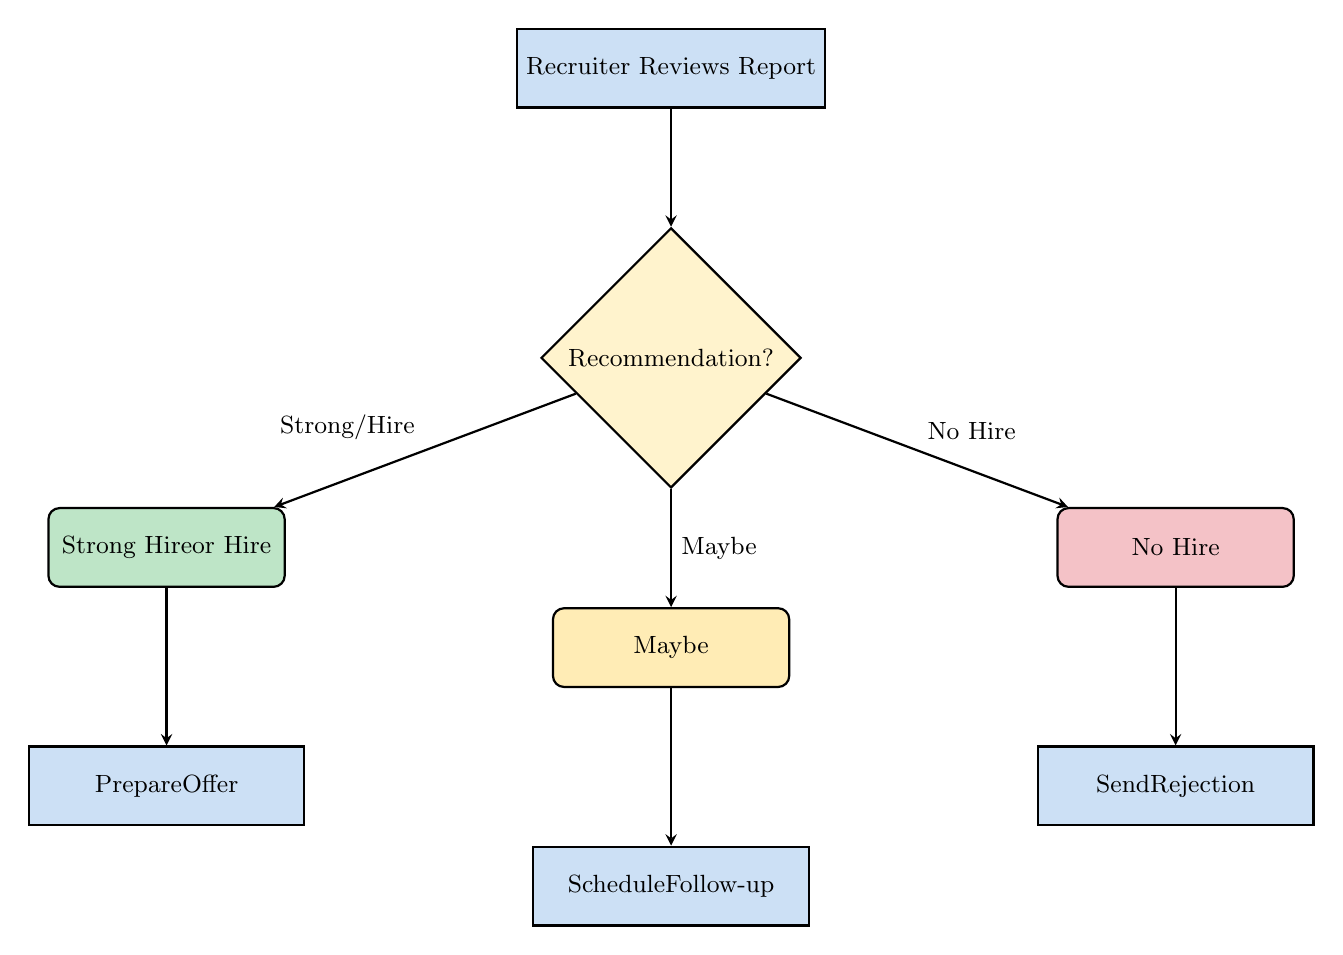
\begin{tikzpicture}[
    node distance=1.5cm,
    every node/.style={font=\small},
    decision/.style={diamond, minimum width=2.5cm, minimum height=1.5cm,
                     text centered, draw=black, fill=warningyellow!20, thick},
    process/.style={rectangle, minimum width=3.5cm, minimum height=1cm,
                    text centered, draw=black, fill=primaryblue!20, thick},
    result/.style={rectangle, rounded corners, minimum width=3cm, minimum height=1cm,
                   text centered, draw=black, thick},
    arrow/.style={->, >=stealth, thick}
]

\node (start) [process] {Recruiter Reviews Report};
\node (decision) [decision, below=of start] {Recommendation?};

\node (stronghire) [result, below left=of decision, xshift=-3cm, fill=successgreen!30] 
    {Strong Hire\\or Hire};
\node (maybe) [result, below=of decision, fill=warningyellow!30] {Maybe};
\node (nohire) [result, below right=of decision, xshift=3cm, fill=dangerred!30] {No Hire};

\node (offer) [process, below=of stronghire, yshift=-0.5cm] {Prepare\\Offer};
\node (followup) [process, below=of maybe, yshift=-0.5cm] {Schedule\\Follow-up};
\node (reject) [process, below=of nohire, yshift=-0.5cm] {Send\\Rejection};

\draw [arrow] (start) -- (decision);
\draw [arrow] (decision) -- node[above left] {Strong/Hire} (stronghire);
\draw [arrow] (decision) -- node[right] {Maybe} (maybe);
\draw [arrow] (decision) -- node[above right] {No Hire} (nohire);
\draw [arrow] (stronghire) -- (offer);
\draw [arrow] (maybe) -- (followup);
\draw [arrow] (nohire) -- (reject);

\end{tikzpicture}
\caption{Hiring Decision Flow}
\end{figure}

\subsection{Decision Path A: HIRE (Strong Hire / Hire)}

\begin{tcolorbox}[colback=successgreen!5,colframe=successgreen,title=\textbf{Hire Decision Process}]

\textbf{Admin Actions:}
\begin{enumerate}
    \item Update application status: "Offer Pending"
    \item Prepare offer letter
    \item Calculate salary package
    \item Schedule onboarding
    \item Notify candidate via email
\end{enumerate}

\textbf{Candidate Receives:}
\begin{itemize}
    \item Offer letter (PDF)
    \item Salary package details
    \item Benefits information
    \item Start date
    \item Onboarding schedule
    \item Welcome package
\end{itemize}

\textbf{Next Steps:}
\begin{itemize}
    \item Candidate accepts/negotiates offer
    \item Background check initiated
    \item Reference checks conducted
    \item Onboarding materials sent
    \item First day scheduled
\end{itemize}

\end{tcolorbox}

\newpage

\subsection{Decision Path B: MAYBE}

\begin{tcolorbox}[colback=warningyellow!5,colframe=warningyellow,title=\textbf{Maybe Decision Process}]

\textbf{Admin Actions:}
\begin{enumerate}
    \item Review red flags and areas for improvement
    \item Discuss with hiring manager
    \item Decide on additional assessment:
    \begin{itemize}
        \item Follow-up technical interview
        \item Take-home coding assignment
        \item System design interview
        \item Cultural fit interview
    \end{itemize}
    \item Schedule next round
    \item Notify candidate
\end{enumerate}

\textbf{Candidate Receives:}
\begin{itemize}
    \item Follow-up interview invitation
    \item Areas to focus on
    \item Timeline for decision
    \item Additional assignment (if applicable)
\end{itemize}

\textbf{Next Steps:}
\begin{itemize}
    \item Candidate completes additional assessment
    \item Admin reviews new data
    \item Final decision: Hire or No Hire
\end{itemize}

\end{tcolorbox}

\vspace{0.5cm}

\subsection{Decision Path C: NO HIRE}

\begin{tcolorbox}[colback=dangerred!5,colframe=dangerred,title=\textbf{No Hire Decision Process}]

\textbf{Admin Actions:}
\begin{enumerate}
    \item Update application status: "Rejected"
    \item Prepare rejection email
    \item Provide feedback (optional)
    \item Archive application
    \item Update ATS
\end{enumerate}

\textbf{Candidate Receives:}
\begin{itemize}
    \item Rejection notification email
    \item Constructive feedback (optional)
    \item Thank you message
    \item Invitation to apply again in future
\end{itemize}

\textbf{System Actions:}
\begin{itemize}
    \item Store interview data for analytics
    \item Update job posting metrics
    \item Add to talent pool (future opportunities)
\end{itemize}

\end{tcolorbox}

\newpage

% ============================================================
\section{Complete Data Flow Summary}
% ============================================================

\subsection{Data Collection Points}

\begin{table}[h!]
\centering
\small
\begin{tabular}{|l|l|l|}
\hline
\textbf{Stage} & \textbf{Data Collected} & \textbf{Count} \\
\hline
Resume Upload & Skills, experience, projects, education & 20+ fields \\
\hline
Face Registration & Facial embeddings (512-dim vector) & 1 vector \\
\hline
Per Question (17 Q\&A) & 
\begin{tabular}{@{}l@{}}
6 behavioral metrics \\
7 vocal metrics \\
4 answer quality metrics
\end{tabular} & 17 metrics × 17 = 289 \\
\hline
Per Coding (3) & 
\begin{tabular}{@{}l@{}}
Compilation status \\
Test cases passed/failed \\
Code efficiency
\end{tabular} & 5 metrics × 3 = 15 \\
\hline
Final Report & 
\begin{tabular}{@{}l@{}}
Overall score \\
4 category scores \\
10+ detailed metrics \\
Red flags \\
Strengths \\
Narratives
\end{tabular} & 30+ fields \\
\hline
\textbf{TOTAL} & & \textbf{350+ data points} \\
\hline
\end{tabular}
\caption{Complete Data Collection Summary}
\end{table}

\subsection{Processing Time Breakdown}

\begin{table}[h!]
\centering
\begin{tabular}{|l|l|l|}
\hline
\textbf{Operation} & \textbf{Time} & \textbf{Notes} \\
\hline
Resume parsing & 2-3 sec & BERT-NER extraction \\
Face registration & 0.5 sec & DeepFace embeddings \\
Face verification & 0.3 sec & Per question \\
Behavioral analysis & 0.5-1 sec & MediaPipe (5 frames) \\
Vocal analysis & 1-2 sec & OpenSMILE + Librosa \\
Answer evaluation & 2-5 sec & LLM API call \\
Coding execution & 1-5 sec & Per test case \\
Report generation & 2-3 sec & Aggregate + narratives \\
\hline
\textbf{Per Question Total} & \textbf{5-8 sec} & Full analysis pipeline \\
\textbf{Full Interview} & \textbf{45-60 min} & 20 questions + coding \\
\hline
\end{tabular}
\caption{Processing Time Analysis}
\end{table}

\newpage

\subsection{System Architecture Diagram}

\begin{figure}[h!]
\centering
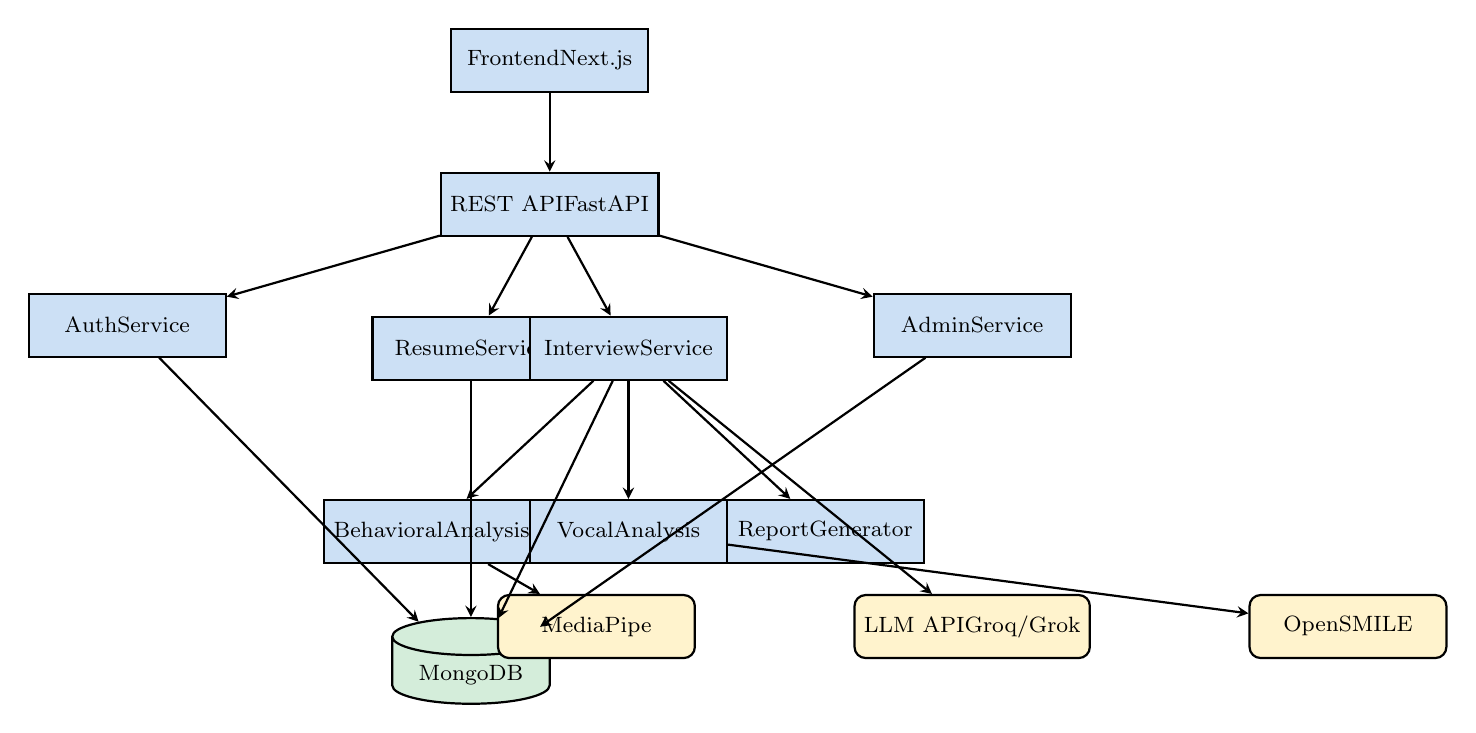
\begin{tikzpicture}[
    node distance=1cm,
    every node/.style={font=\footnotesize},
    component/.style={rectangle, minimum width=2.5cm, minimum height=0.8cm,
                      text centered, draw=black, fill=primaryblue!20, thick},
    database/.style={cylinder, shape border rotate=90, aspect=0.3,
                     minimum width=2cm, minimum height=0.8cm,
                     draw=black, fill=successgreen!20, thick},
    external/.style={rectangle, rounded corners, minimum width=2.5cm, minimum height=0.8cm,
                     text centered, draw=black, fill=warningyellow!20, thick},
    arrow/.style={->, >=stealth, thick}
]

% Frontend
\node (frontend) [component] {Frontend\\Next.js};

% API Layer
\node (api) [component, below=of frontend] {REST API\\FastAPI};

% Services
\node (auth) [component, below left=of api, xshift=-2cm] {Auth\\Service};
\node (resume) [component, below=of api, xshift=-1cm] {Resume\\Service};
\node (interview) [component, below=of api, xshift=1cm] {Interview\\Service};
\node (admin) [component, below right=of api, xshift=2cm] {Admin\\Service};

% Interview Sub-services
\node (behavioral) [component, below=of interview, xshift=-2.5cm, yshift=-0.5cm] 
    {Behavioral\\Analysis};
\node (vocal) [component, below=of interview, yshift=-0.5cm] {Vocal\\Analysis};
\node (report) [component, below=of interview, xshift=2.5cm, yshift=-0.5cm] 
    {Report\\Generator};

% Database
\node (db) [database, below=of resume, yshift=-2cm] {MongoDB};

% External APIs
\node (llm) [external, below=of admin, yshift=-2cm] {LLM API\\Groq/Grok};
\node (mediapipe) [external, left=of llm, xshift=-1cm] {MediaPipe};
\node (opensmile) [external, right=of llm, xshift=1cm] {OpenSMILE};

% Arrows
\draw [arrow] (frontend) -- (api);
\draw [arrow] (api) -- (auth);
\draw [arrow] (api) -- (resume);
\draw [arrow] (api) -- (interview);
\draw [arrow] (api) -- (admin);

\draw [arrow] (interview) -- (behavioral);
\draw [arrow] (interview) -- (vocal);
\draw [arrow] (interview) -- (report);

\draw [arrow] (auth) -- (db);
\draw [arrow] (resume) -- (db);
\draw [arrow] (interview) -- (db);
\draw [arrow] (admin) -- (db);

\draw [arrow] (behavioral) -- (mediapipe);
\draw [arrow] (vocal) -- (opensmile);
\draw [arrow] (interview) -- (llm);

\end{tikzpicture}
\caption{System Architecture}
\end{figure}

\newpage

% ============================================================
\section{Key Metrics \& Performance}
% ============================================================

\subsection{Evaluation Metrics Summary}

\begin{table}[h!]
\centering
\begin{tabular}{|l|l|l|}
\hline
\textbf{Category} & \textbf{Metrics} & \textbf{Range} \\
\hline
\multirow{6}{*}{Behavioral} & Eye Contact & 0-100 \\
& Head Stability & 0-100 \\
& Facial Engagement & 0-100 \\
& Fidgeting Score & 0-100 \\
& Confidence Posture & 0-100 \\
& Attention Span & 0-100 \\
\hline
\multirow{7}{*}{Vocal} & Vocal Confidence & 0-100 \\
& Speech Clarity & 0-100 \\
& Pitch Variance & 0-100 \\
& Speech Rate & 0-100 \\
& Pause Pattern & 0-100 \\
& Tone Consistency & 0-100 \\
& Communication & 0-100 \\
\hline
\multirow{4}{*}{Answer Quality} & Relevance Score & 0-10 \\
& Depth Score & 0-10 \\
& Accuracy Score & 0-100 \\
& Communication Score & 0-10 \\
\hline
\multirow{2}{*}{Coding} & Test Cases Passed & Count \\
& Compilation Success & Boolean \\
\hline
\end{tabular}
\caption{All Evaluation Metrics}
\end{table}

\subsection{Score Interpretation Guide}

\begin{table}[h!]
\centering
\begin{tabular}{|l|l|l|}
\hline
\textbf{Score Range} & \textbf{Rating} & \textbf{Interpretation} \\
\hline
90-100 & Excellent & Outstanding performance \\
80-89 & Very Good & Strong performance \\
70-79 & Good & Satisfactory performance \\
60-69 & Fair & Acceptable with concerns \\
50-59 & Poor & Below expectations \\
0-49 & Very Poor & Significant issues \\
\hline
\end{tabular}
\caption{Score Interpretation}
\end{table}

\newpage

% ============================================================
\section{Security \& Privacy}
% ============================================================

\subsection{Data Security Measures}

\begin{itemize}
    \item \textbf{Authentication:} JWT tokens with expiration
    \item \textbf{Authorization:} Role-based access control (RBAC)
    \item \textbf{Password Security:} Bcrypt hashing
    \item \textbf{Data Encryption:} HTTPS/TLS for all API calls
    \item \textbf{Database Security:} MongoDB authentication \& encryption
    \item \textbf{Video/Audio:} Not stored permanently, only metrics
    \item \textbf{Face Data:} Embeddings only, original images deleted
    \item \textbf{API Security:} Rate limiting, CORS protection
\end{itemize}

\subsection{Privacy Compliance}

\begin{tcolorbox}[colback=primaryblue!5,colframe=primaryblue,title=\textbf{GDPR Compliance}]
\textbf{Data Minimization:}
\begin{itemize}
    \item Only collect necessary data
    \item Video/audio not stored permanently
    \item Only metrics and scores stored
\end{itemize}

\textbf{User Rights:}
\begin{itemize}
    \item Right to access (view own reports)
    \item Right to deletion (delete account \& data)
    \item Right to rectification (update profile)
    \item Right to data portability (export reports)
\end{itemize}

\textbf{Consent:}
\begin{itemize}
    \item Explicit consent before interview
    \item Clear explanation of data usage
    \item Option to decline recording
\end{itemize}
\end{tcolorbox}

\subsection{Anti-Cheating Measures}

\begin{enumerate}
    \item \textbf{Face Verification:} Every question
    \item \textbf{Multiple Face Detection:} Alert if >1 face detected
    \item \textbf{Coaching Detection:} Audio anomaly analysis
    \item \textbf{Screen Monitoring:} Tab switching detection (optional)
    \item \textbf{Code Plagiarism:} Compare with known solutions
    \item \textbf{Response Time:} Flag suspiciously fast answers
\end{enumerate}

\newpage

% ============================================================
\section{Conclusion}
% ============================================================

\subsection{System Benefits}

\begin{tcolorbox}[colback=successgreen!5,colframe=successgreen,title=\textbf{Key Benefits}]

\textbf{For Recruiters:}
\begin{itemize}
    \item \textbf{Time Savings:} 80\% reduction in evaluation time
    \item \textbf{Consistency:} Standardized evaluation criteria
    \item \textbf{Data-Driven:} Objective metrics replace bias
    \item \textbf{Scalability:} Handle 10x more interviews
    \item \textbf{Quality:} Comprehensive 350+ data points
\end{itemize}

\textbf{For Candidates:}
\begin{itemize}
    \item \textbf{Fair Assessment:} Objective evaluation
    \item \textbf{Real-time Feedback:} See metrics during interview
    \item \textbf{Flexibility:} Interview from anywhere
    \item \textbf{Transparency:} Understand evaluation criteria
    \item \textbf{Fast Process:} Results within 1-2 days
\end{itemize}

\textbf{For Companies:}
\begin{itemize}
    \item \textbf{Better Hires:} Multi-dimensional assessment
    \item \textbf{Cost Reduction:} Automated evaluation
    \item \textbf{Compliance:} GDPR-compliant system
    \item \textbf{Analytics:} Track hiring metrics
    \item \textbf{Integration:} Works with existing ATS
\end{itemize}

\end{tcolorbox}

\subsection{Success Metrics}

\begin{table}[h!]
\centering
\begin{tabular}{|l|l|}
\hline
\textbf{Metric} & \textbf{Target} \\
\hline
Interview Completion Rate & >95\% \\
Evaluation Accuracy & >90\% \\
Time per Interview & <60 minutes \\
Recruiter Satisfaction & >4.5/5 \\
Candidate Satisfaction & >4.0/5 \\
False Positive Rate & <5\% \\
False Negative Rate & <5\% \\
System Uptime & >99.9\% \\
\hline
\end{tabular}
\caption{System Success Metrics}
\end{table}

\subsection{Future Enhancements}

\begin{itemize}
    \item \textbf{Multi-language Support:} Interview in 50+ languages
    \item \textbf{Historical Benchmarking:} Compare with successful hires
    \item \textbf{Custom Rubrics:} Per-role evaluation criteria
    \item \textbf{AI Coaching Mode:} Help candidates prepare
    \item \textbf{Integration:} Connect with major ATS systems
    \item \textbf{Mobile App:} Interview from phone/tablet
    \item \textbf{Analytics Dashboard:} Hiring trends \& insights
    \item \textbf{Video Proctoring:} Advanced anti-cheating
\end{itemize}

\vspace{1cm}

\begin{center}
\Large\textbf{End of Pipeline Documentation}
\end{center}

\end{document}
